\documentclass{homework}
\author{Tomás Pérez}
\class{Mathematical Biostatistics Boot Camp 1}
\date{\today}
\title{Theory \& Notes}

\graphicspath{{./media/}}

\begin{document} \maketitle

\section{Part 1}
\section{Part 2}
\subsection{Week 1}

\subsubsection{Hypothesis testing}

Hypothesis testing is concerned with making decisions using data. We label a null hypothesis as $H_0$. The null hypothesis is assumed true and statistical evidence is required to rejected in favor of an alternative hypothesis. 

For example, a respiratory disturbance index of more than 30 events/hour is considered evidence of severe sleep disorder breathing. Suppose that in a sample of 100 overweight subjects with other risk factors for sleep disordered breathing at a sleep clinic, the mean RDI was 32 events/hour with a standard deviation of 10 events/hour.

We might want to test the hypothesis that 

\begin{itemize}
    \item $H_0 : \mu = 30$ 
    \item $H_a : \mu > 30$ 
\end{itemize}

where $\mu$ is the population mean RDI. The alternative hypothesis are typically of the form $<,> or \neq$. Note that there four possible outcome of our statistical decision process

\begin{tabular}{ |p{1cm}||p{5cm}|p{5cm}|  }
 \hline
 \multicolumn{3}{|c|}{Statistical decision process} \\
 \hline
 Truth& $H_0$ & $H_a$\\
 \hline
 $H_0$  & Correctly accept null & Type I error\\
 $H_a$ &  Type II error & Correctly reject null\\
 \hline
\end{tabular} \\

\begin{itemize}
    \item The type I error rate is a false positive \textit{ie.} the mistaken rejection of a (true) null hypothesis. 
    \item The type II error rate is a false negative \textit{ie.} the mistaken acceptance of a (false) null hypothesis, we failed to reject a false $H_0$.
\end{itemize}

Let $\alpha$ denote the type I error rate, the probability of rejecting the null hypothesis when, in fact, then null hypothesis is correct. We'd like to minimise this kind of error. Considering our previous example, a reasonable strategy would reject the null hypothesis if $\Bar{X}$ was larger than some constant $C \in \mathds{R}_{+}$. Typically, $C$ is chosen so that the probability of a Type I error $\alpha$ is 0.05

For example, the probability of a Type I error and according to the Central Limit Theorem we have  

\begin{align}
        .05 = \mathds{P}\bigg(\Bar{X}\geq C \bigg| \mu = 30 \bigg) \\
        = \mathds{P}\bigg(\frac{\Bar{X}-30}{10/\sqrt{100}}\geq \frac{C-30}{10/\sqrt{100}} \bigg| \mu = 30 \bigg) \\
        =  \mathds{P}\bigg(Z\geq \frac{C-30}{10/\sqrt{100}}\bigg)
\end{align}

Hence $\frac{C-30}{1}=1.645$ implying $C=31.645$. Now, since our mean is $32$ we reject the null hypothesis. We can plot a the 95th percentile of the standard normal distribution with the following R routine:
\begin{lstlisting}[language=R]
xval <-  seq(-3.2, 3.2, length=1000)
yval <- dnorm(xval)
plot(xval, yval, type="l", axes=TRUE, frame=FALSE, lwd=3, xlab="", ylab="")
x <- seq(qnorm(.95), 3.2, length=1000)
polygon(c(x,rev(x)), c(dnorm(x), rep(0, length(x))), col="salmon")
text(mean(x), mean(dnorm(x))+0.2, "5%", cex=2)
text(qnorm(.95), .01, "1.645",cex=2)
\end{lstlisting}. 

which outputs the following graph

\begin{figure}
    \centering
    \includegraphics[scale=0.4]{figs/95th percentile of a gaussian.png} 
    \caption{R-generated plot of the standard normal distribution $\mathcal{N}(0,1)$,  in the [-3.2, 3.2] range. The shaded polygon represents the 95th percentile (which is given by $x=1.645$) of a standard normal distribution. }
    \label{fig:my_label}
\end{figure}

In general, we don't convert $C$ back to its original scale. We would just reject it because the Z-score, how many standard error units the sample mean is above the hypothesised mean, is greater than $1.645$ \textit{ie. }

$$
\frac{32-30}{10/\sqrt{100}} = 2 > 1.645.
$$

Our mean is two standard error units away from the hypothesised mean 

We can codify these rules for a normal Z test, assuming the data is gaussian or that the Central Limit Theorem is a good enough approximation to apply, as follows:

Let $H_0 : \mu = \mu_0$ be the null hypothesis, then let 
\begin{itemize}
    \item $H_1: \mu < \mu_0$
    \item $H_2: \mu \neq \mu_0$
    \item $H_3: \mu > \mu_0$
\end{itemize}

where the test statistic $TS = \frac{\Bar{X}-\mu_0}{S/\sqrt{a}}$ (expressing the mean in standard error units), where $S/\sqrt{a}$ is the standard error. Thus, we reject the null hypothesis when 

\begin{itemize}
\item $H_1: TS \leq -Z_{1-\alpha}$ \textit{ie.} we reject $H_0$ in favour of $H_1$ if our sample mean is enough below $\mu_0$,
    \item $H_2: |TS| \geq  Z_{1-\alpha/2}$ \textit{ie.} we reject in favour of $H_2$ if our sample mean is enough too different from $\mu_0$ (either too large or too small)\footnote{In this case, we look at the $(1-\alpha/2)\times 100\%$ error rate, we divide the probability of a type I error into half of it being accidentally rejected because of sample mean being too large and the other half of it being accidentally rejected because the sample mean is }, 
    \item $H_3: TS \geq Z_{1-\alpha}$ \textit{ie.} we reject in favour of $H_3$ if our sample mean is enough above $\mu_0$.
\end{itemize}

The region of TS values for which the null hypothesis is rejected is the rejection region. In the case of $H_1$, the upper normal quantile and above is the rejection region, for $H_2$ it's the negative quantile and below or the upper quantile and above and finally, in the case of $H_3$, the normal quantile and below is the rejection region.

We can graphically represent the second case, the case of a two-sided tail test, with the following R routine

\begin{lstlisting}[language=R]
xval <-  seq(-3.2, 3.2, length=1000)
yval <- dnorm(xval)

plot(xval, yval, type = "l", axes=TRUE, frame=FALSE, lwd = 3, xlab="", ylab= "")
x <- seq(qnorm(.975), 3.2, length = 100)
polygon(c(x, rev(x)), c(dnorm(x), rep(0,length(x))), col="salmon")
text(mean(x), mean(dnorm(x))+0.2, "2.5%", cex=2)
text(qnorm(.975), .01, "1.96",cex=2)

x <- seq(-3.2, qnorm(0.025), length=100)
polygon(c(x, rev(x)), c(dnorm(x), rep(0,length(x))), col="salmon")
text(mean(x), mean(dnorm(x))+0.2, "2.5%", cex=2)
text(qnorm(.025), .01, "1.96",cex=2)
text(0, dnorm(0)/5, "95%",cex=2)
\end{lstlisting}

\begin{figure}
    \centering
    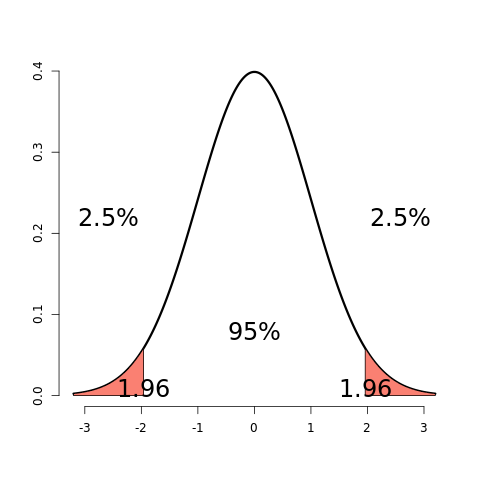
\includegraphics[scale = 0.4]{figs/two sided tail test.png}
    \caption{Two sided tail test presenting a standard normal $\mathcal{N}(0,1)$ distribution. We're going to reject $H_0$ if our test statistic is above $1.96$ -which has a 2.5\% chance under the null hypothesis- and we're going to reject $H_0$ if our test statistic is below $-1.96$ -which also has a 2.5\% chance under the null hypothesis-. Thus the union of those two events has a 5\% chance under the null hypothesis. }
    \label{fig:my_label}
\end{figure}

In hypothesis testing, we fix the $\alpha$ (type I error value) to be low. So if we reject the null hypothesis, either our model is wrong or there is a low probability that we made and error. We haven't fixed the probability of a type II error $\beta$, therefore we tend to say "fail to reject $H_0$" rather than accepting $H_0$. In general, less is known about the type II error. Statistical significance is not the same as scientific significance. 

\subsubsection{Two sided tests}

The Z-test requires the assumption of the Central Limit theorem and for $n$ to be large enough for the CLT to apply. If $n$ is mall, then a Gossett's $T$ test is performed exactly in the same way with the normal quantiles being replaced by the appropriate Student's $T$ quantiles and $n-1$ degrees of freedom. 

The probability of rejecting a false null hypothesis is called \textbf{power}. The statistical power of a dichotomic (binary) hypothesis test is the probability that the test correctly rejects the null hypothesis $H_0$ when a specific alternative hypothesis $H_1$ is true\footnote{Remember that the probability of rejecting a true null hypothesis is the type I error rate and is set to be small whilst the probability of failing to reject (this is the mistaken acceptance) a false null hypothesis is called a type II error rate. The power is $1-\beta$.}. A high value of power is good thing, we want to reject a false null hypothesis but it's not an easy to manipulate quantity in an experiment. One way to combat this issue is, prior to conducting the study, to do a power calculation of the sample size to obtain a certain level of power using guesses for the standard deviation and the hypothesised significant effect.

For example, suppose that $n=16$ (rather than 100) in our previous example. Instead of using a Z-test, we use a Student's $T$-test. Then 

$$
.05 = \mathds{P}\bigg(\frac{\Bar{X}-30}{s/\sqrt{16}} \geq t_{1-\alpha, 15} \bigg| \mu = 30\bigg)
$$

where $s/\sqrt{16}$ is the estimated standard error, where $t_{1-\alpha, 15}$ is t-quantile. Then our test statistic is now $\sqrt{16}\frac{32-30}{10} = .8$, while the critical value is $t_{1-\alpha, 15} = 1.75$. Thus, we fail to reject the null hypothesis. Remember that T has a heavier tail distribution than the normal distribution.

We are now interested in a two sided test. We are interested in studying if our hypothesised mean is significantly larger than $30$ or significantly smaller than $30$. That is, we want to test he alternative hypothesis $H_a: \mu \neq 30$. Then

$$
\alpha = \mathds{P}\bigg(\bigg|\frac{\Bar{X}-30}{s/\sqrt{16}}\bigg| > t_{1-\alpha/2, 15}\bigg| \mu = 30\bigg),
$$

that is: we'll reject $H_0$ is the test statistic (0.8) is either too large or two small with the critical value being calculated using $\alpha/2$. In our example, this critical value is $2.13$ so we fail to reject it\footnote{We note that, if the data are iid Gaussians, then $\frac{X-\mu}{s/\sqrt{n}} \sim t_{n-1}$} The previous calculation can be understood with the following R routine 

\begin{lstlisting}[language=R]
xval <-  seq(-4, 4, length=1000)
yval <- dt(xval, 15)
plot(xval, yval, type = "l", axes=TRUE, frame=FALSE, lwd = 3, xlab="", ylab= "")
x <- seq(qt(.975, 15), 4, length=100)
polygon(c(x, rev(x)), c(dt(x,15), rep(0,length(x))), col="salmon")
text(mean(x), mean(dt(xval, 16-1))+0.2, "2.5%", cex=2)
text(qt(.975,15), .01, "2.13",cex=2)
x <- seq(-3.2, qt(.025,16), length=100)
polygon(c(x, rev(x)), c(dt(x,15), rep(0,length(x))), col="salmon")
text(mean(x), mean(dt(xval, 16-1))+0.2, "2.5%", cex=2)
text(qt(.025,15), .01, "2.13",cex=2)
text(0, dt(0,15)/5, "95%", cex=2)
\end{lstlisting}

which outputs figure \ref{fig: two sided Student's T test}.

\begin{figure}
    \centering
    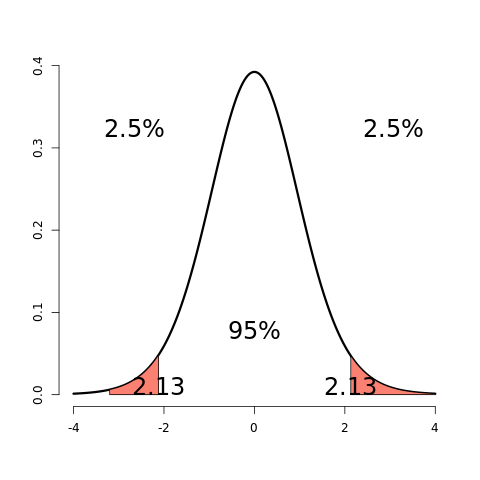
\includegraphics[scale=0.4]{figs/two sided T test.png}
    \caption{We calculate our normalised test statistic $\frac{\Bar{X}-\mu}{s/\sqrt{n}}$ and the probability that the absolute value of said statistic is bigger than $2.13$ \textit{ie.} the probability that the statistic is too large positive than $2.13$ is 2.5\% or too small negative than $-2.13$ is 2.5\%. In our case, the probability that the test statistic lies in the rejection region is 5\%. For the $T$ distributionwith 15 degrees of freedom, the 97.5th quantile is 2.13 and the 2.5th quantile is $-2.13$. }
    \label{fig: two sided Student's T test}
\end{figure}

\subsubsection{Confidence intervals and P values}

Consider testing $H_0 : \mu = \mu_0$ versus $H_a : \mu \neq \mu_0$. Take the set of all possible values for which we fail to reject $H_0$, this set is a $(1-\alpha)\times 10\%$ confidence interval for $\mu$, these are the value for $\mu$ that are supportable as null hypotheses (those are reasonable numbers for $\mu$). This rule works both ways, if a $(1-\alpha)\times 10\%$ contains $\mu_0$, then we fail to reject $H_0$.

Consider that we don't reject $H_0$ if our test statistic behaves as follows:

$$
\bigg|\frac{\Bar{X}-\mu}{s/\sqrt{n}}\bigg| \leq t_{1-\alpha/2, n-1},
$$

which implies 

$$
|\Bar{X}-\mu| \leq t_{1-\alpha/2, n-1} s/\sqrt{n}
$$

which, in turn, implies that 

$$
\bar{X} - t_{1-\alpha/2, n-1} \frac{s}{\sqrt{n}} < \mu_0 < \bar{X} + t_{1-\alpha/2, n-1} \frac{s}{\sqrt{n}}.
$$

This states that if $\mu_0$ lies inside the confidence interval, the we've failed to reject $H_0$ and this argument is reversible. This establishes a duality between confidence intervals and two-sided hypotheses tests. If we create a 95\% confidence interval, it conveys more information than the result of a hypothesis test because we can do the hypothesis test and gives a sense of what values for $\mu_0$ are well supported, helping to reduce the gap between statistical significance and scientific significance. 

In our previous example, we rejected the one-sided test when $\alpha = .05$, would we reject it if $.01$ or $.001$?

The smallest value for $\alpha$ that you still reject the null hypothesis is called the \textbf{attained significance level}. This equivalent, but philosophically different, from the \textbf{P-value}.
The P-value (same number but different concept) is the probability, under the null hypothesis, of obtaining evidence as extreme or more extreme than would be observed by chance alone, where chance is governed by the null distribution. If the P-value is small, then either $H_0$ is true and we have observed a rare event, given that the null hypothesis is true, or $H_0$ is false. It quantifies whether or not getting a test statistic as or more extreme than you observed was rare under the null hypothesis. If it's rare, then that casts some doubt on the veracity of the null hypothesis. 

In our example, the $T$ statistic was $0.8$. What's the probability of getting a $T$ statistic as large as $0.8$? This can be computed with the following R code 

\begin{lstlisting}[language=R]
pt(0.8, 15, lower.tail = FALSE) 

In [1]:  0.218099
\end{lstlisting}

where \texttt{pt} stands for $T$ probability, \texttt{lower.tail = FALSE} indicates we want a value above $0.8$, not lower. This works out to be $P = 22\% > \alpha = 5\%$, which is entirely reasonable because we failed to reject the null hypothesis. 

\begin{itemize}
    \item If the P-value is larger than $\alpha$, we fail to reject $H_0$. 
    \item If the P-value is smaller than $\alpha$, we reject $H_0$
\end{itemize}

This can be understood via the following R routine 

\begin{lstlisting}[language=R]
pt(0.8, 15, lower.tail=FALSE)
xval <-  seq(-4, 4, length=1000)
yval <- dt(xval, 15)
plot(xval, yval, type = "l", axes=TRUE, frame=FALSE, lwd = 3, xlab="", ylab= "")
x <-  seq(.8, 4, length=100)
polygon(c(x, rev(x)), c(dt(x,15), rep(0,length(x))), col="salmon")
text(mean(x), mean(dt(xval, 16-1))+0.2, "22%", cex=2)
text(.8, .01, "0.8",cex=2)
\end{lstlisting}

which outputs figure \ref{fig: P-value T statistic}

\begin{figure}
    \centering
    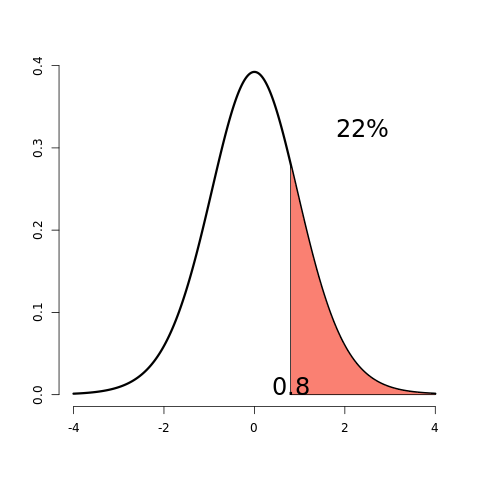
\includegraphics[scale = .4]{figs/P-value T statistic.png}
    \caption{Our statistic $\frac{\bar{X}-\mu}{s/\sqrt{n}}$ turned out to be .8. The probability of being .8 or larger for a Student's $T$ distribution with 15 degrees of freedom is $22\%$. Since this number is larger than $\alpha = 5\%$, we would fail to reject $H_0$. }
    \label{fig: P-value T statistic}
\end{figure}

By reporting a P-value, the reader can perform a hypothesis test at whatever $\alpha$ level he or she chooses. Again, is the P-value is less than $\alpha$, we reject the null hypothesis.

For two sided hypothesis test, double the smaller of the two one sided hypothesis test P-values. \\ 

Criticisms of the P value:

\begin{itemize}
    \item P values only consider significance, unlike confidence intervals making it harder to distinguish practical significance from statistical significance.
    \item Absolute measures of the rareness of an event are not good measures of the evidence for or against a hypothesis.
\end{itemize}

\subsubsection{Power}

Power is the probability of rejecting the null hypothesis when it's false. And, as the name suggests, it's a desirable quality, the more power, the more reliable the test is. A type II error is failing to reject the null hypothesis when it's false. Thus, by their definitions, power + type II error rate ($\beta$) sum to one. Thus we define $\textnormal{Power} = 1- \beta$.

Consider the example involving RDI. The null hypothesis is $H_0 : \mu = 30$ versus $H_a : \mu > 30$. Then power is calculated under the alternative hypothesis, as follows  

$$
\mathds{P}\bigg(\frac{\bar{X}-30}{s/\sqrt{n}} > t_{1-\alpha, n-1} \bigg | \mu = \mu_a\bigg).
$$

The power of the test is the probability that the $T$ statistic lies in the rejection region. If this normalised mean was greater than the $t_{1-\alpha, n-1}$ quantile, then we reject the null hypothesis. Note that this quantity is calculated not under the assumption of the null hypothesis but rather calculated under the assumption of the alternative hypothesis. Note that this function depends on the specific value of $\mu_a$ and we notice that, as $\mu \rightarrow 30$, power approaches $\alpha$.

\subsubsection{Calculating Power}

Assume that $n$ is large and we know $\sigma$, then

\begin{align*}
    1- \beta = 
\end{align*}

\end{document}
